\documentclass[11pt]{article}

\usepackage{apacite}

\title{My first replicable Paper}
\author{
        MyFirstName MyLastName\\
        Evans School of Public Policy and Governance\\
        University of Washington\\
        Seattle, WA 98115, \underline{United States}\\
        \texttt{greatguy@uw.edu}
}
\date{\today}


\usepackage{Sweave}
\begin{document}
\Sconcordance{concordance:PaperInR_4.tex:PaperInR_4.Rnw:%
1 15 1 1 0 31 1 1 2 4 0 1 2 4 1 1 2 12 0 1 2 10 1 1 5 17 0 1 2 7 1 1 6 %
1 2 6 1 1 5 15 0 1 2 5 1 1 2 4 0 1 2 3 1 1 2 4 0 1 2 8 1 1 2 31 0 1 2 %
12 1}


\maketitle


\begin{abstract}
This is an example on how to make a reproducible paper. We are using R from Rstudio, creating an RSweave document. This is a nice start to create a nice paper and get an A+. The next sections will show the steps taken.
\end{abstract}

\section{Introduction}\label{intro}
This is my intro to my great paper, I will explain the cool things I can do with my new `computational thinking' powers combined with some Latex.

This is my nice intro to my great paper, 
I will explain the cool things I can do with my new `computational thinking' powers combined with some Latex.



This is my nice intro to my great paper, 
I will explain the cool things 
I can do with my new `computational thinking' 
powers
combined with some Latex.

\section{Explaining Labels}\label{outline}

Sections may use a label\footnote{In fact, you can have a label wherever you think a future reference to that content might be needed.}. This label is needed for referencing. For example the next section has label \emph{datas}, so you can reference it by writing: As we see in section \ref{datas}.

\section{Data analysis}\label{datas}

Here you can explain how to get the data:

\begin{Schunk}
\begin{Sinput}
> states=read.csv("https://goo.gl/So48s5")
\end{Sinput}
\end{Schunk}

\subsection{Exploration}\label{eda}

Here, I start exploring the data. The first step is to know what variables I have, and in what scale they are:

\begin{Schunk}
\begin{Soutput}
'data.frame':	51 obs. of  8 variables:
 $ state                : Factor w/ 51 levels "Alabama",""..
 $ satMean              : int  991 920 932 1005 897 959 89..
 $ satDemand            : num  0.08 0.41 0.26 0.06 0.47 0...
 $ k12ExpenditurePupil  : int  3627 8330 4309 3700 4491 50..
 $ incomeHouseholsMedian: num  27.5 48.3 32.1 24.6 41.7 ...
 $ diplomaHsAdults      : num  0.669 0.866 0.787 0.663 0.7..
 $ collegeDegreeAdults  : num  0.157 0.23 0.203 0.133 0.23..
 $ region               : Factor w/ 4 levels "Midwest","N"..
\end{Soutput}
\end{Schunk}

% bullets

A next step demands:
\begin{itemize}
  \item Knowing the \emph{central} and \emph{dispersion} values.
  \item Visualizing the variables of interest.
\end{itemize}

Except for the column \emph{state}, we can compute the centrality and spread measures for the other variables in the data. I will do that in Table \ref{measures} in the next page.

% Table created by stargazer v.5.2 by Marek Hlavac, Harvard University. E-mail: hlavac at fas.harvard.edu
% Date and time: ����, 1�� 04, 2018 - 9:59:14
\begin{table}[!htbp] \centering 
  \caption{Mean and Spread values} 
  \label{measures} 
\begin{tabular}{@{\extracolsep{5pt}}lccccc} 
\\[-1.8ex]\hline 
\hline \\[-1.8ex] 
Statistic & \multicolumn{1}{c}{N} & \multicolumn{1}{c}{Mean} & \multicolumn{1}{c}{St. Dev.} & \multicolumn{1}{c}{Min} & \multicolumn{1}{c}{Max} \\ 
\hline \\[-1.8ex] 
satMean & 51 & 944.098 & 66.935 & 832 & 1,093 \\ 
satDemand & 51 & 0.358 & 0.262 & 0.040 & 0.810 \\ 
k12ExpenditurePupil & 51 & 5,235.961 & 1,401.155 & 2,960 & 9,259 \\ 
incomeHouseholsMedian & 51 & 33.957 & 6.423 & 23.465 & 48.618 \\ 
diplomaHsAdults & 51 & 0.763 & 0.056 & 0.643 & 0.866 \\ 
collegeDegreeAdults & 51 & 0.200 & 0.042 & 0.123 & 0.333 \\ 
\hline \\[-1.8ex] 
\end{tabular} 
\end{table} 
As you saw, my Table \ref{measures} is nice. As you, saw the mean of the variable \emph{satMean} is 944.098039215686. Now let's use a boxplot to explore location:

%%%%%%%
% figure 

\begin{figure}[h]
\centering
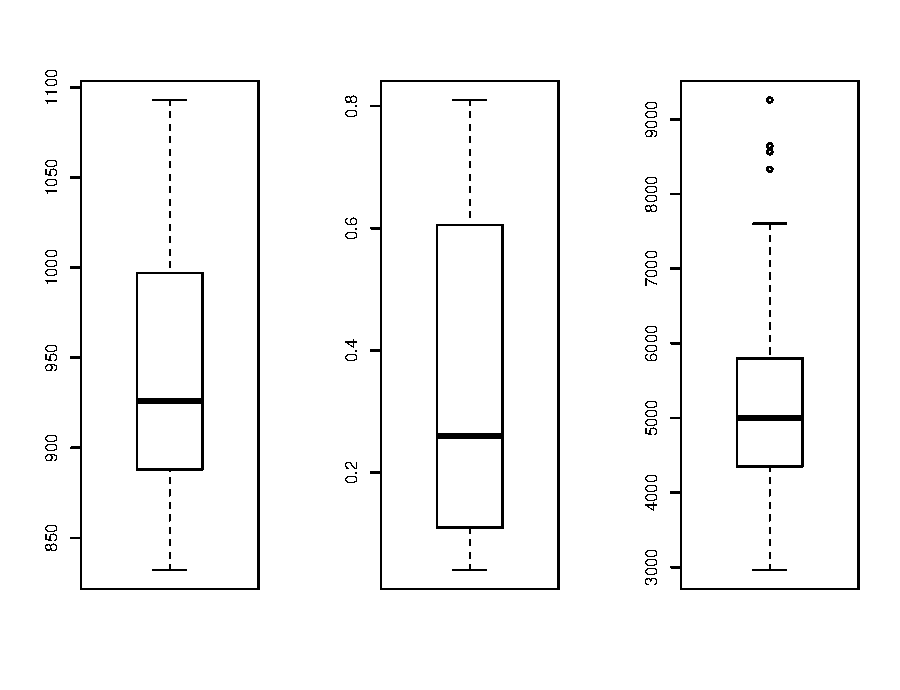
\includegraphics{PaperInR_4-location}
\caption{Location of values}
\label{plot_boxplots}
\end{figure}


As we have a categorical variable, we could create a frequency table:

% Table created by stargazer v.5.2 by Marek Hlavac, Harvard University. E-mail: hlavac at fas.harvard.edu
% Date and time: ����, 1�� 04, 2018 - 9:59:18
\begin{table}[!htbp] \centering 
  \caption{Distribution of Region} 
  \label{table_region} 
\begin{tabular}{@{\extracolsep{5pt}} cc} 
\\[-1.8ex]\hline 
\hline \\[-1.8ex] 
Region & Frequency \\ 
\hline \\[-1.8ex] 
Midwest & $12$ \\ 
N. East & $9$ \\ 
South & $17$ \\ 
West & $13$ \\ 
\hline \\[-1.8ex] 
\end{tabular} 
\end{table} 


\subsection{Modeling}\label{model}

Here, I propose that the amount of money spent for child per state in the US has an effect on the mean average pupils in a state get in SAT:
\begin{Schunk}
\begin{Sinput}
> reg1=lm(satMean~k12ExpenditurePupil, data = states)
\end{Sinput}
\end{Schunk}

Here, I modify the previous model; while I insist that the amount of money spent for child per state in the US has an effect on the mean average pupils in a state get in SAT; I will control the effect the demand per state (as demand were equal accross states). Then,

Model 2: 
\begin{Schunk}
\begin{Sinput}
> reg2=lm(satMean~k12ExpenditurePupil+satDemand, data = states)
\end{Sinput}
\end{Schunk}

I have the results, but have not display them, let's do it in the coming subsection
%%%%%%%
%% better way coming here!!!!!

\subsection{Modeling nicely}\label{modelnice}

What about this:

% Table created by stargazer v.5.2 by Marek Hlavac, Harvard University. E-mail: hlavac at fas.harvard.edu
% Date and time: ����, 1�� 04, 2018 - 9:59:18
\begin{table}[!htbp] \centering 
  \caption{Regression Models} 
  \label{regmods} 
\begin{tabular}{@{\extracolsep{5pt}}lcc} 
\\[-1.8ex]\hline 
\hline \\[-1.8ex] 
 & \multicolumn{2}{c}{\textit{Dependent variable:}} \\ 
\cline{2-3} 
\\[-1.8ex] & \multicolumn{2}{c}{satMean} \\ 
\\[-1.8ex] & (1) & (2)\\ 
\hline \\[-1.8ex] 
 Dollars per Student & $-$0.022$^{***}$ & 0.009$^{**}$ \\ 
  & (0.006) & (0.004) \\ 
  & & \\ 
 Share taking SAT &  & $-$253.770$^{***}$ \\ 
  &  & (22.491) \\ 
  & & \\ 
 Constant & 1,060.732$^{***}$ & 989.807$^{***}$ \\ 
  & (32.701) & (18.396) \\ 
  & & \\ 
\hline \\[-1.8ex] 
Observations & 51 & 51 \\ 
R$^{2}$ & 0.217 & 0.786 \\ 
Adjusted R$^{2}$ & 0.201 & 0.777 \\ 
Residual Std. Error & 59.814 (df = 49) & 31.623 (df = 48) \\ 
F Statistic & 13.615$^{***}$ (df = 1; 49) & 88.009$^{***}$ (df = 2; 48) \\ 
\hline 
\hline \\[-1.8ex] 
\textit{Note:}  & \multicolumn{2}{r}{$^{*}$p$<$0.1; $^{**}$p$<$0.05; $^{***}$p$<$0.01} \\ 
\end{tabular} 
\end{table} 
\clearpage

\section{Explaining Citations}\label{citation}


Citing requires a \emph{bib} file with all the books. You can create it from Zotero, and then add it here with the command \emph{cite}. For example, open the file named `GovernanceAnalytics' and write the name of the author here.
\cite{suo_meowmeow_2018}
\cite{magallanes_reyes_introducing_2017}

\bibliographystyle{apacite} 
\bibliography{Gov} %you can change this 'bibfile' name.
\end{document}
